\documentclass[a4paper]{article}

\usepackage{../styles/new-style}
\usepackage{float}
\usepackage{tikz}

\newcommand{\hmwkTitle}{Minimaalse kaaluga toesuspuu ja rändkaupmehe ülesanne} % Assignment title
\newcommand{\hmwkClass}{Algoritmid ja andmestruktuurid} % Course/class

\begin{document}

\textbf{Kodutöö esitamise tähtaeg: 17. detsember, 23:59}

{\center
\subsection*{Minimaalse kaaluga toesuspuu}
}

Olgu $G = (V, E)$ sidus ja kaalutud servadega graaf. Graafi $G$ toesuspuuks nimetatakse puud $T = (V, E')$, kus $E' \subseteq E$. Teisiti öeldes on toesuspuu $T$ selline graafi $G$ alamgraaf, mis ühendab kõiki tema tippe, kuid ei sisalda tsükleid. Igal sidusal graafil leidub toesuspuu.

Graafi $G$ minimaalseks toesuspuuks nimetatakse sellist toesuspuud, mille servade kaalude summa on vähim. On teada mitmeid efektiivseid algoritme toesuspuu leidmiseks. Selles praktikumis vaatleme kahte ahnet
algoritmi: Primi algoritmi ja Kruskali algoritmi.

\begin{figure}[H]
\centering
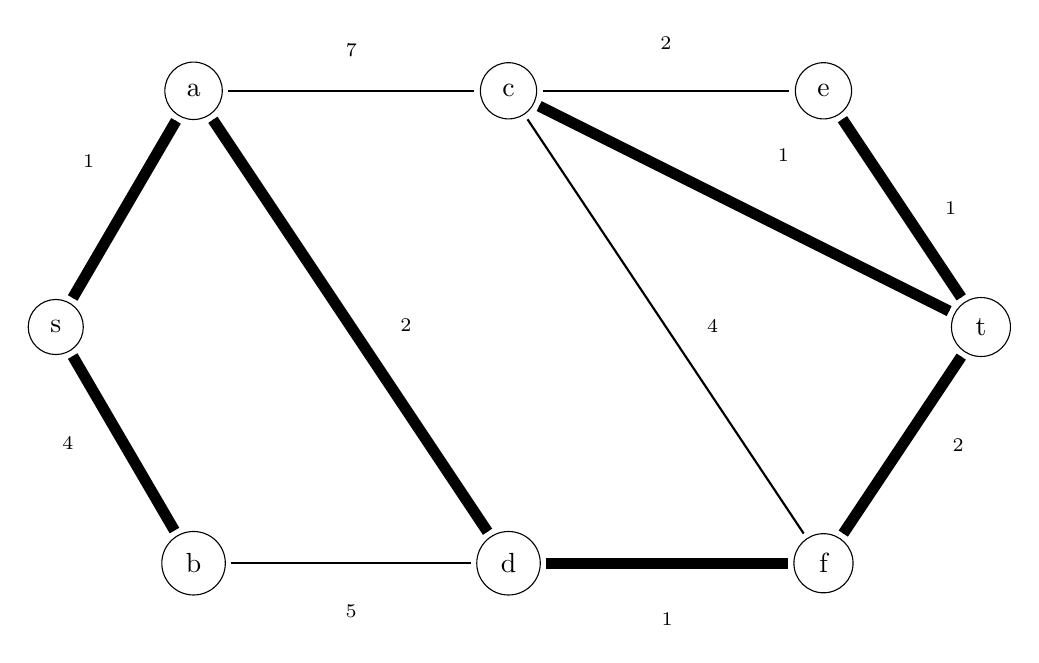
\begin{tikzpicture}
\node[shape= circle, draw, inner sep=5pt] (s) at (1.25,0) {s};
\node[shape = circle, draw, inner sep=5pt] (a) at (3,3) {a};
\node[shape = circle, draw, inner sep=5pt] (b) at (3,-3) {b};
\node[shape = circle, draw, inner sep=5pt] (c) at (7,3) {c};
\node[shape = circle, draw, inner sep=5pt] (d) at (7,-3) {d};
\node[shape = circle, draw, inner sep=5pt] (e) at (11,3) {e};
\node[shape = circle, draw, inner sep=5pt] (f) at (11,-3) {f};
\node[shape = circle, draw, inner sep=5pt] (t) at (13,0) {t};
\path[thick, shorten <=2pt,shorten >=2pt, every node/.style={font=\scriptsize}]
(s) edge node[label={[label distance=5]120:}] {} (a)
(f) edge node[label={[label distance=7.5]0:}] {} (t)
(e) edge node[label={[label distance=5]0:}] {} (t)
(a) edge node[label={[label distance=5]90:7}] {} (c)
(b) edge node[label={[label distance=7.5]270:5}] {} (d)
(d) edge node[label={[label distance=7.5]0:}] {} (a)
(d) edge node[label={[label distance=7.5]270:}] {} (f)
(c) edge node[label={[label distance=7.5]90:2}] {} (e)
(c) edge node[label={[label distance=7.5]60:}] {} (t)
(c) edge node[label={[label distance=7.5]0:4}] {} (f);

\path[line width = 4pt, shorten <=2pt,shorten >=2pt, every node/.style={font=\scriptsize}]
(s) edge node[label={[label distance=5]120:$1$}] {} (a)
(s) edge node[label={[label distance=7.5]180:4}] {} (b)
(f) edge node[label={[label distance=7.5]0:$2$}] {} (t)
(e) edge node[label={[label distance=5]0:$1$}] {} (t)
(d) edge node[label={[label distance=7.5]0:$2$}] {} (a)
(d) edge node[label={[label distance=7.5]270:$1$}] {} (f)
(c) edge node[label={[label distance=7.5]60:$1$}] {} (t);
\end{tikzpicture}
\caption{Paksemad jooned tähistavad antud graafi minimaalset aluspuud.}
\end{figure}


\begin{problem}

\textbf{Ülesanne 1}
Implementeerida minimaalse toesuspuu leidmine kas Primi või Kruskali algoritmiga vastavalt liidesele \textit{MinimumSpanningTreeAlgorithm}.
\end{problem}

{\center
\subsection*{Rändkaupmehe ülesanne}
}

Olgu meile antud teatud linnad ja lühimad teed iga kahe linna vahel. Rändkaupmehe ülesanne küsib, milline on lühim teekond, mis läbib kõiki linnu ja jõuab lõpuks algpunkti tagasi.

Probleemi sõnastus formaalsemalt võiks olla selline: \textit{olgu meile antud täisgraaf (iga tipp on ühendatud iga teise tipuga) $G$, mille servad on kaalutud. Leida vähima kaaluga tsükkel, mis sisaldab kõiki tippe.}

Seni ei ole teada ühtegi efektiivset algoritmi, mis suudaks suvalise täisgraafi korral anda sellele probleemile täpse vastuse. (Efektiivse algoritmi leidmine lahendaks ka ühe olulisema küsimuse informaatikas. Vaata:\newpage \href{https://en.wikipedia.org/wiki/P_versus_NP_problem}{$P$ vs $NP$}). Teada on aga mitmeid algoritme, mis annavad ligikaudseid tulemusi. Näiteks on võimalik leida minimaalne toesuspuu ja see eesjärjestus süvitsi läbida.

\begin{problem}
\textbf{Ülesanne 2}

Leida lähend rändkaupmehe ülesandele kasutades minimaalse kaaluga toesuspuud. Implementeerida vastavalt liidesele \textit{ApproximateTravelingSalesman}.
\end{problem}

Liidesed on kättesaadavad aaddressil \url{https://github.com/ut-aa/aa2016-lab8}.

\end{document}